\documentclass[12pt,letterpaper]{article}
\usepackage{graphicx}
\usepackage{ifpdf}

\usepackage{multicol}
\usepackage{tikz}

\usepackage{amssymb}
\usepackage{amsmath}

\usepackage{float}

\usepackage{caption}
\usepackage{subcaption}

\usepackage{hyperref}
% \usepackage{cite}

%\usepackage[backend=bibtex]{biblatex}
%\bibliography{bibliografia} 

\hypersetup{
    colorlinks=true,
    linkcolor=black,
    citecolor = black,
%     filecolor=magenta,      
    urlcolor=black,
%     pdftitle={GSP Toolbox Manual},
    bookmarks=true
%     pdfpagemode=FullScreen,
}

\usepackage[spanish]{babel}

\usepackage{fancyhdr}
 
\pagestyle{fancy}
\fancyhf{}
\rhead{Isaac Ayala Lozano\\194520009 \hspace{2 em}   \textbf{\#2}}
\lhead{}
\fancyfoot[R]{\thepage}

\begin{document}
\section{Problema 1}

Se presentan las condiciones de simulación para el péndulo invertido con resorte en la tabla \ref{table: ip initial conditions}. 

\begin{table}[h]
\begin{center}
\centering
\begin{tabular}{cccc}
\hline
Tiempo inicial ($t_0$) & 0  & Posición inicial ($x_0$) & $1$ \\
%\hline
Tiempo final ($t_f$) & 10 & Velocidad inicial ($\dot{x}_0$)& $1$\\
Masa del vehículo ($m_c$) & $3$ &  Posición angular inicial ($\theta_0$) & $\dfrac{3 \pi}{4}$\\
Masa del péndulo ($m_p$) & 1 & Velocidad angular inicial ($\dot{\theta}_0$)& $0$\\
Constante de gravedad ($g$) & $9.81$ & Longitud ($l$) & $1.5$ \\
&  & Constante de resorte ($k$) & $0.5$ \\
\hline
\end{tabular}
\end{center}
 \caption{Condiciones de simulación.}
 \label{table: ip initial conditions}
\end{table}


\subsection{Caso 1: $F=0$}

Del comportamiento de $x$, $\dot{x}$, $\theta$ y $\dot{theta}$ observado en las figuras \ref{fig: dp x theta force 0} y \ref{fig: dp dx dtheta force 0} notamos que el comportamiento del modelo no considera al resorte.
Esto es conocido, ya que al revisar el modelo propuesto, se hizo una omisión del efecto que éste tiene sobre el potencial $V$ en el sistema.

Los diagramas de fase en las figuras  \ref{fig: dp phase x dx force 0} y \ref{fig: dp phase theta dtheta force 0} observamos el comportamiento de un péndulo invertido que 
oscila sin indicación alguna de llegar a un punto de equilibrio.

\begin{figure}[h]
 \centering
 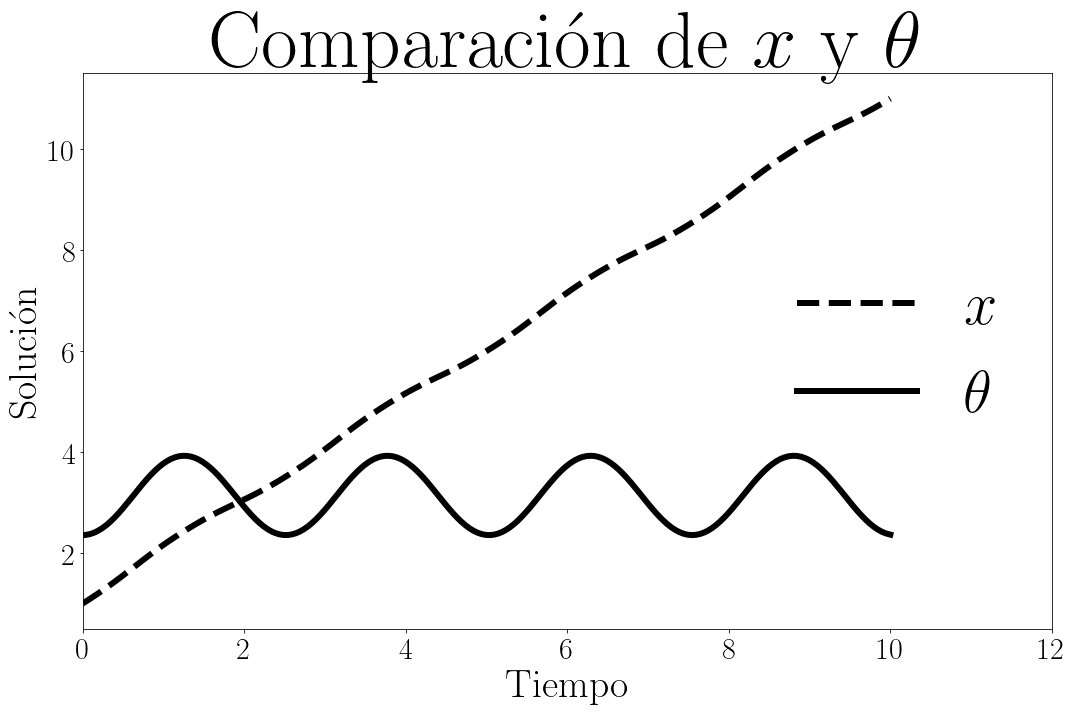
\includegraphics[scale=0.3]{img/dp_x_theta_f0.png}
 % dp_x_theta_f0.png: 1072x712 px, 72dpi, 37.83x25.12 cm, bb=0 0 1072 712
 \caption{Diagramas de $x$ y $\theta$ para $F=0$.}
 \label{fig: dp x theta force 0}
\end{figure}

\begin{figure}[h]
 \centering
 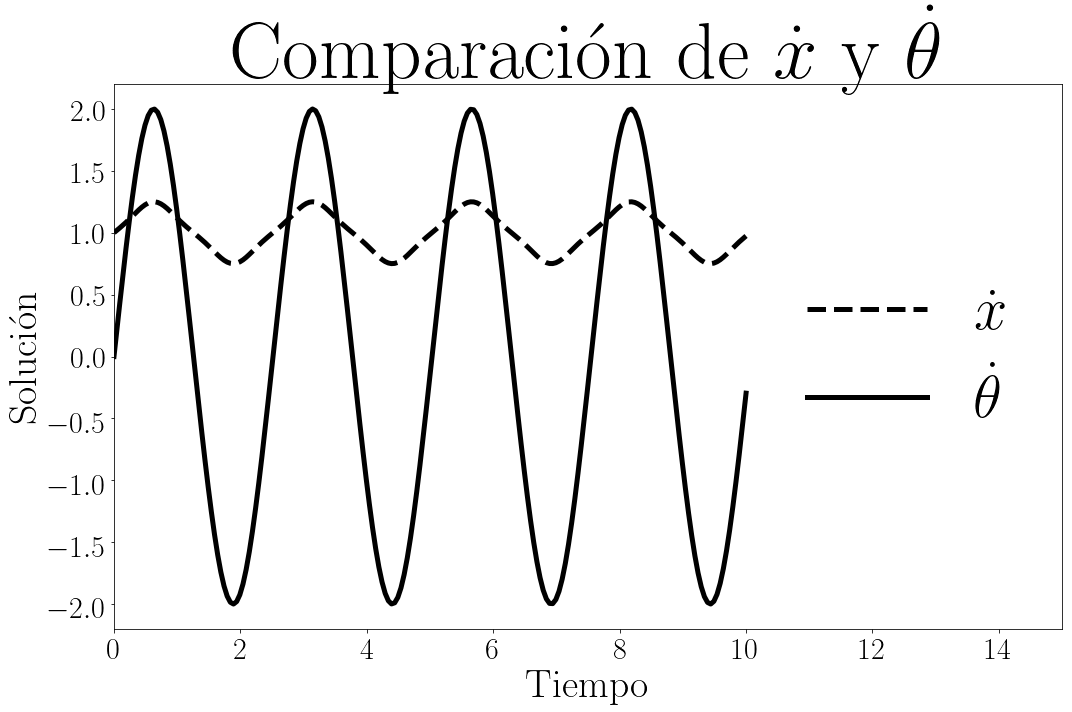
\includegraphics[scale=0.4]{img/dp_dx_dtheta_f0.png}
 % dp_x_theta_f0.png: 1072x712 px, 72dpi, 37.83x25.12 cm, bb=0 0 1072 712
 \caption{Diagramas de $\dot{x}$ y $\dot{\theta}$ para $F=0$.}
 \label{fig: dp dx dtheta force 0}
\end{figure}

\begin{figure}[h]
 \centering
 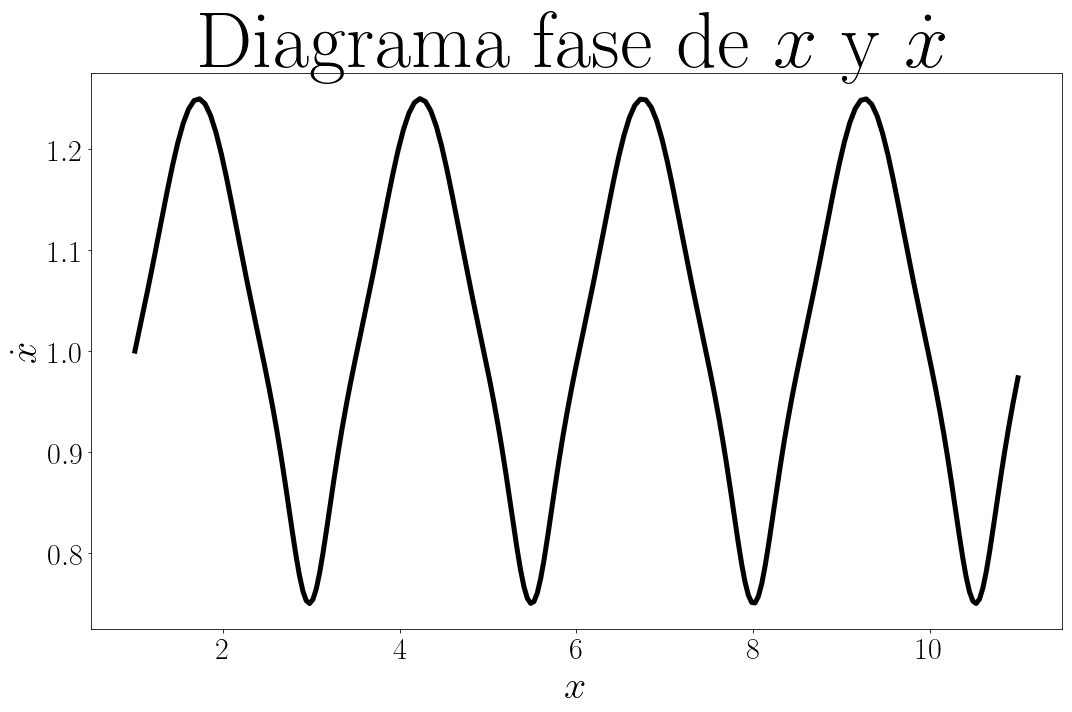
\includegraphics[scale=0.2]{img/dp_phase_x_dx_f0.png}
 % dp_x_theta_f0.png: 1072x712 px, 72dpi, 37.83x25.12 cm, bb=0 0 1072 712
 \caption{Diagrama fase de $x$ y $\dot{x}$ para $F=0$.}
 \label{fig: dp phase x dx force 0}
\end{figure}

\begin{figure}[h]
 \centering
 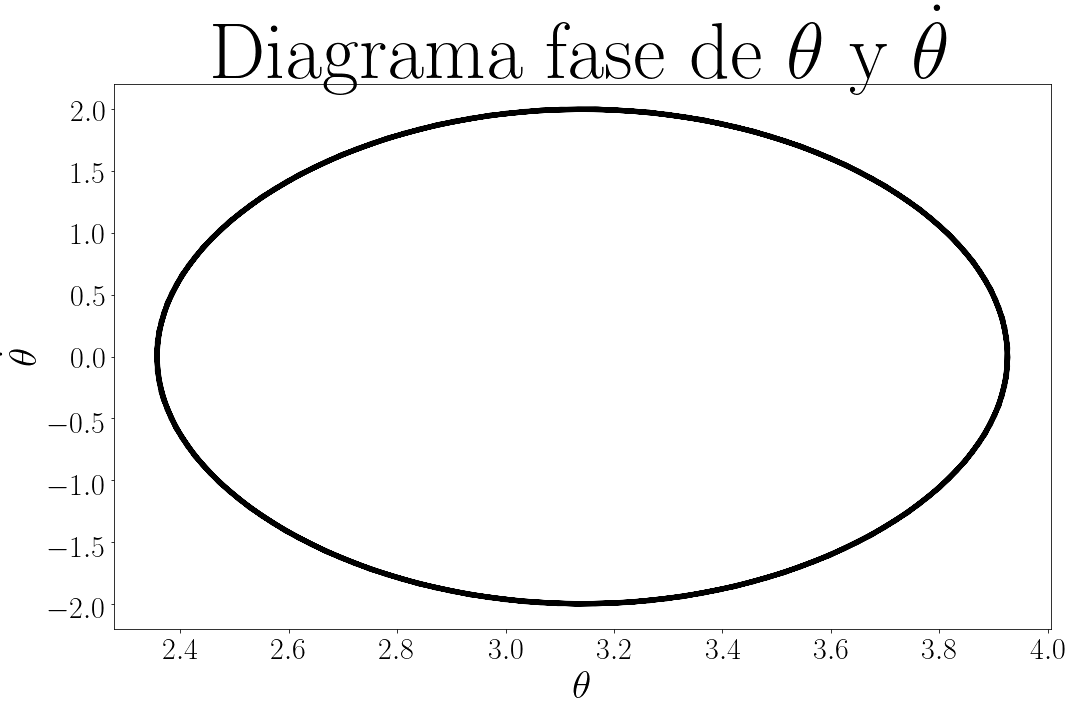
\includegraphics[scale=0.2]{img/dp_phase_theta_dtheta_f0.png}
 % dp_x_theta_f0.png: 1072x712 px, 72dpi, 37.83x25.12 cm, bb=0 0 1072 712
\caption{Diagrama fase de $\theta$ y $\dot{\theta}$ para $F=0$.}
 \label{fig: dp phase theta dtheta force 0}
\end{figure}

\pagebreak

\subsection{Caso 2: $F=1$}

De manera similar al caso 1, las figuras \ref{fig: dp x theta force 1} y 
\ref{fig: dp dx dtheta force 1} muestran el comportamiento del sistema ante una fuerza introducida. Los diagramas de fase de las figuras \ref{fig: dp phase x dx force 1} y \ref{fig: dp phase theta dtheta force 1} presentan un comportamiento similar al caso 1. 

\begin{figure}[h]
 \centering
 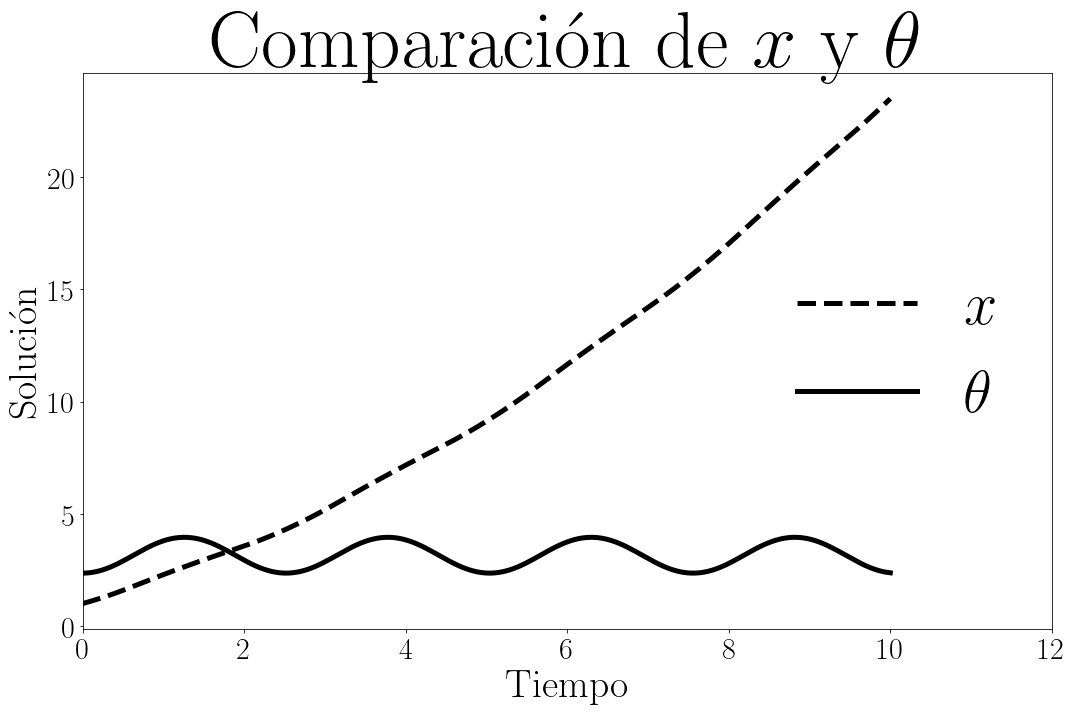
\includegraphics[scale=0.4]{img/dp_x_theta_f1.png}
 % dp_x_theta_f0.png: 1072x712 px, 72dpi, 37.83x25.12 cm, bb=0 0 1072 712
 \caption{Diagramas de $x$ y $\theta$ para $F=1$.}
 \label{fig: dp x theta force 1}
\end{figure}

\begin{figure}[h]
 \centering
 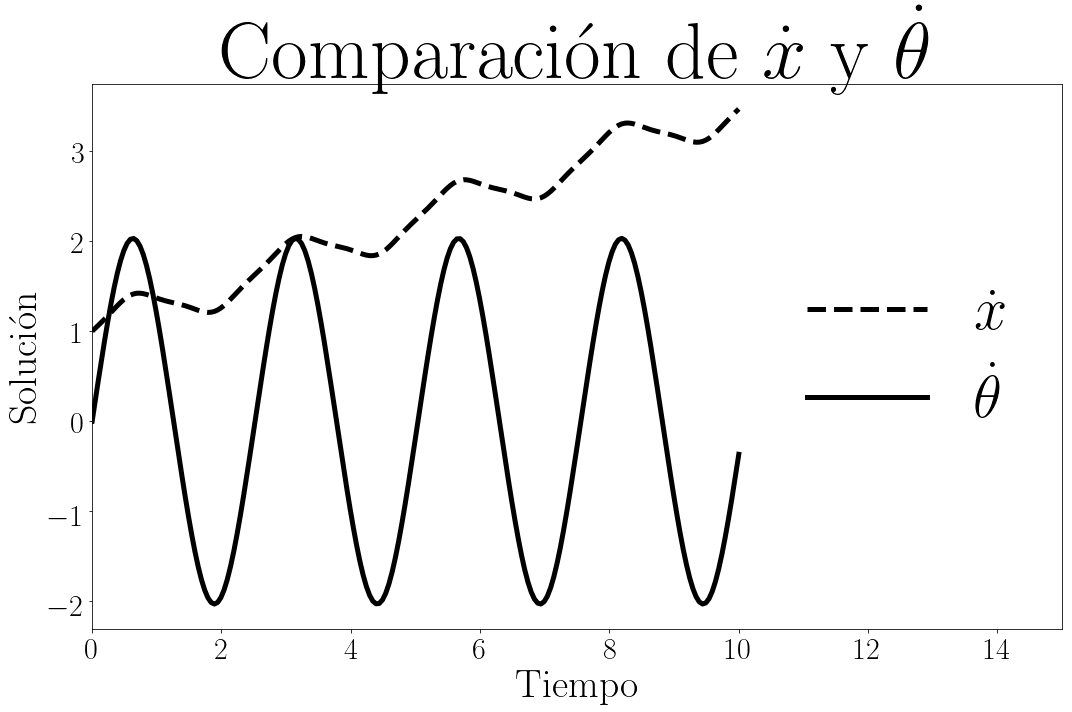
\includegraphics[scale=0.4]{img/dp_dx_dtheta_f1.png}
 % dp_x_theta_f0.png: 1072x712 px, 72dpi, 37.83x25.12 cm, bb=0 0 1072 712
 \caption{Diagramas de $\dot{x}$ y $\dot{\theta}$ para $F=1$.}
 \label{fig: dp dx dtheta force 1}
\end{figure}

\begin{figure}[h]
 \centering
 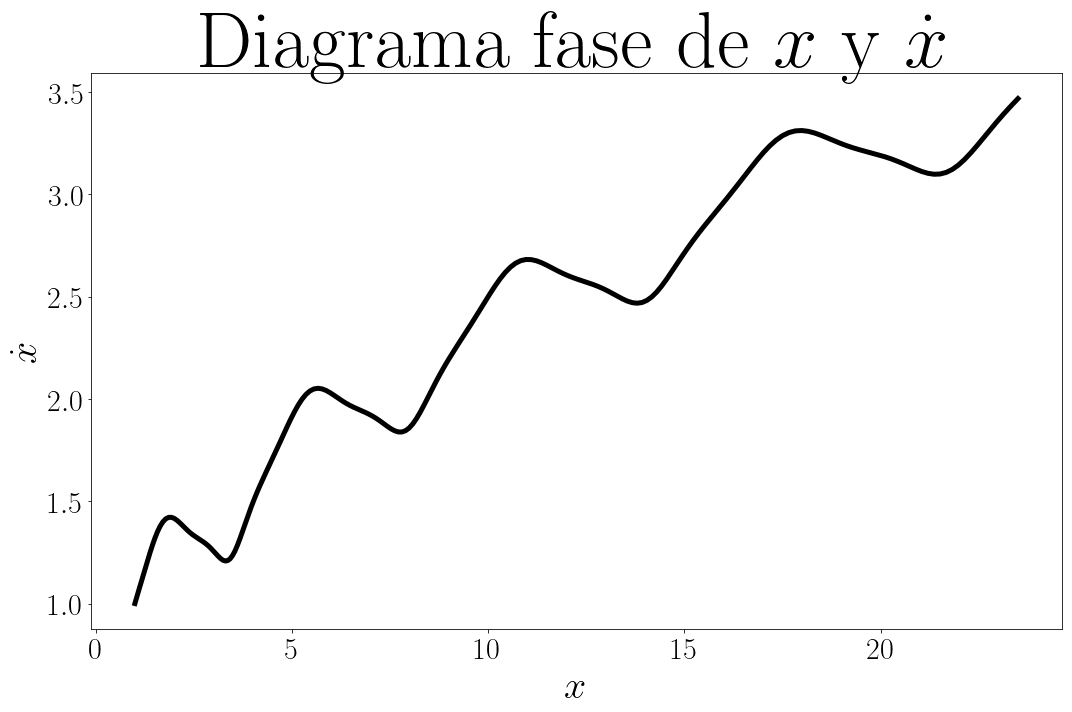
\includegraphics[scale=0.2]{img/dp_phase_x_dx_f1.png}
 % dp_x_theta_f0.png: 1072x712 px, 72dpi, 37.83x25.12 cm, bb=0 0 1072 712
 \caption{Diagrama fase de $x$ y $\dot{x}$ para $F=1$.}
 \label{fig: dp phase x dx force 1}
\end{figure}

\begin{figure}[h]
 \centering
 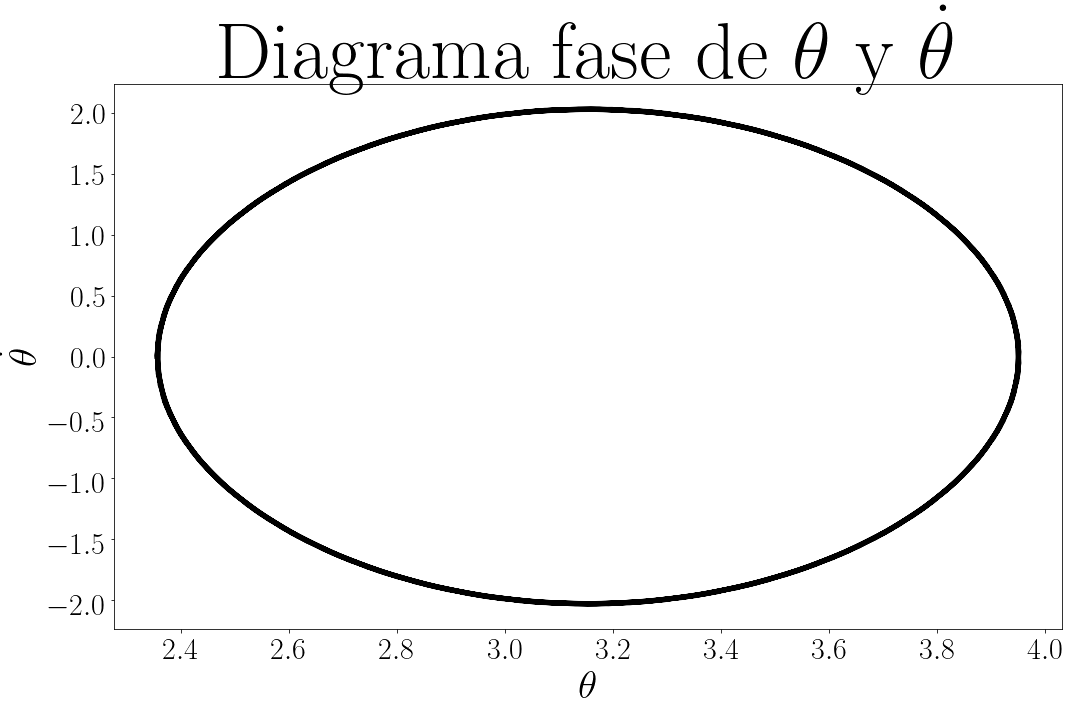
\includegraphics[scale=0.2]{img/dp_phase_theta_dtheta_f1.png}
 % dp_x_theta_f0.png: 1072x712 px, 72dpi, 37.83x25.12 cm, bb=0 0 1072 712
\caption{Diagrama fase de $\theta$ y $\dot{\theta}$ para $F=1$.}
 \label{fig: dp phase theta dtheta force 1}
\end{figure}

\pagebreak


% +++++++++++++++++++++++++++++
% +++++++++++++++++++++++++++++
% +++++++++++++++++++++++++++++

\section{Problema 2}

Se presentan las condiciones de simulación para el péndulo invertido con resorte en la tabla \ref{table: sp initial conditions}. 

\begin{table}[h]
\begin{center}
\centering
\begin{tabular}{cccc}
\hline
Tiempo inicial ($t_0$) & 0  & Posición inicial ($x_0$) & $1$ \\
%\hline
Tiempo final ($t_f$) & 10 & Velocidad inicial ($\dot{x}_0$)& $1$\\
 Constante de resorte ($k$) & $0.5$ &  Posición angular inicial ($\theta_0$) & $1$\\
Masa del péndulo ($m_p$) & 1 & Velocidad angular inicial ($\dot{\theta}_0$)& $1$\\
Constante de gravedad ($g$) & $9.81$ & Longitud ($l$) & $1.5$ \\
%  &  & & \\
\hline
\end{tabular}
\end{center}
 \caption{Condiciones de simulación.}
 \label{table: sp initial conditions}
\end{table}

\subsection{Caso 1: $F=0$}

Para el modelo de péndulo simple conectado a un resorte las variables $x$, $\dot{x}$, $\theta$ y $\dot{theta}$ presentan el comportamiento mostrado en las figuras \ref{fig: sp x theta force 0} y \ref{fig: sp dx dtheta force 0}. Nuevamente, se observa un comportamiento inconsistene en el sistema debido a la 
omisión del efecto del resorte en el potencial de energía $V$ del sistema.

Las figuras  \ref{fig: sp phase x dx force 0} y \ref{fig: sp phase theta dtheta force 0} muestran
los diagramas fases correspondientes.

\begin{figure}[h]
 \centering
 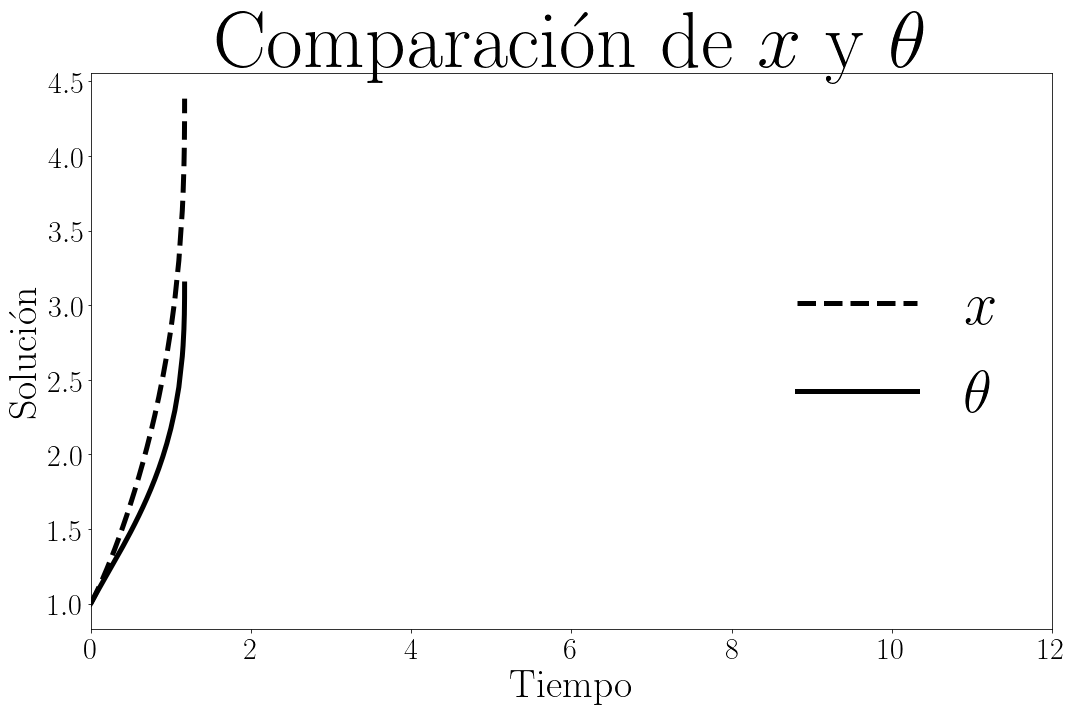
\includegraphics[scale=0.4]{img/sp_x_theta_f0.png}
 % dp_x_theta_f0.png: 1072x712 px, 72dpi, 37.83x25.12 cm, bb=0 0 1072 712
 \caption{Diagramas de $x$ y $\theta$ para $F=0$.}
 \label{fig: sp x theta force 0}
\end{figure}

\begin{figure}[h]
 \centering
 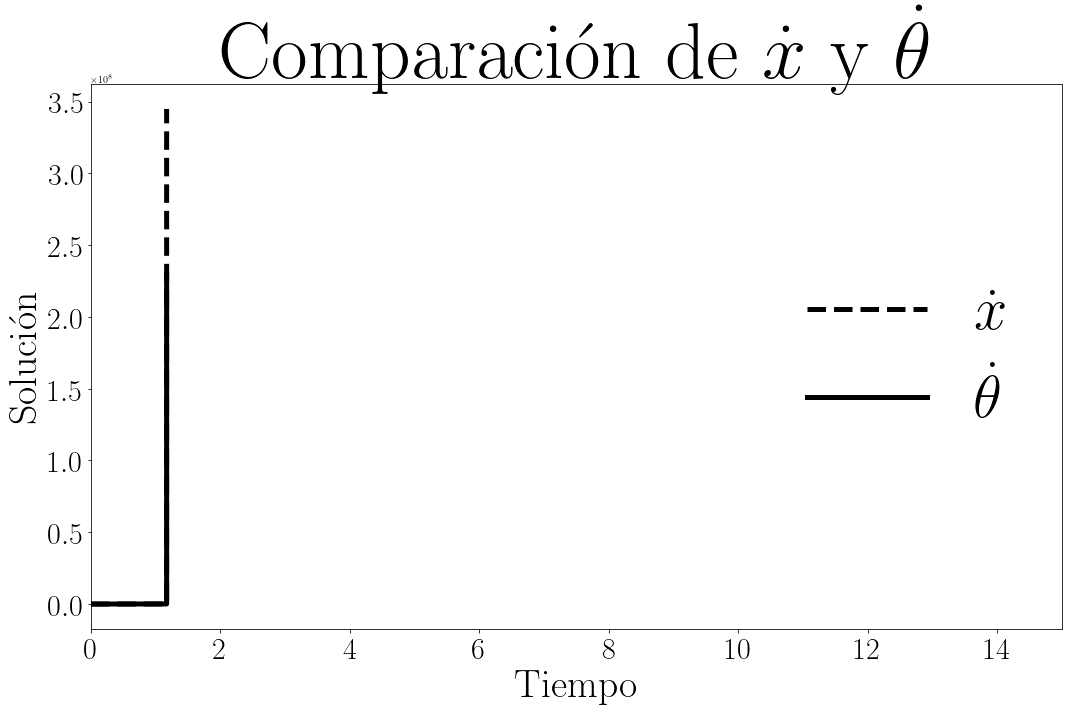
\includegraphics[scale=0.4]{img/sp_dx_dtheta_f0.png}
 % dp_x_theta_f0.png: 1072x712 px, 72dpi, 37.83x25.12 cm, bb=0 0 1072 712
 \caption{Diagramas de $\dot{x}$ y $\dot{\theta}$ para $F=0$.}
 \label{fig: sp dx dtheta force 0}
\end{figure}

\begin{figure}[h]
 \centering
 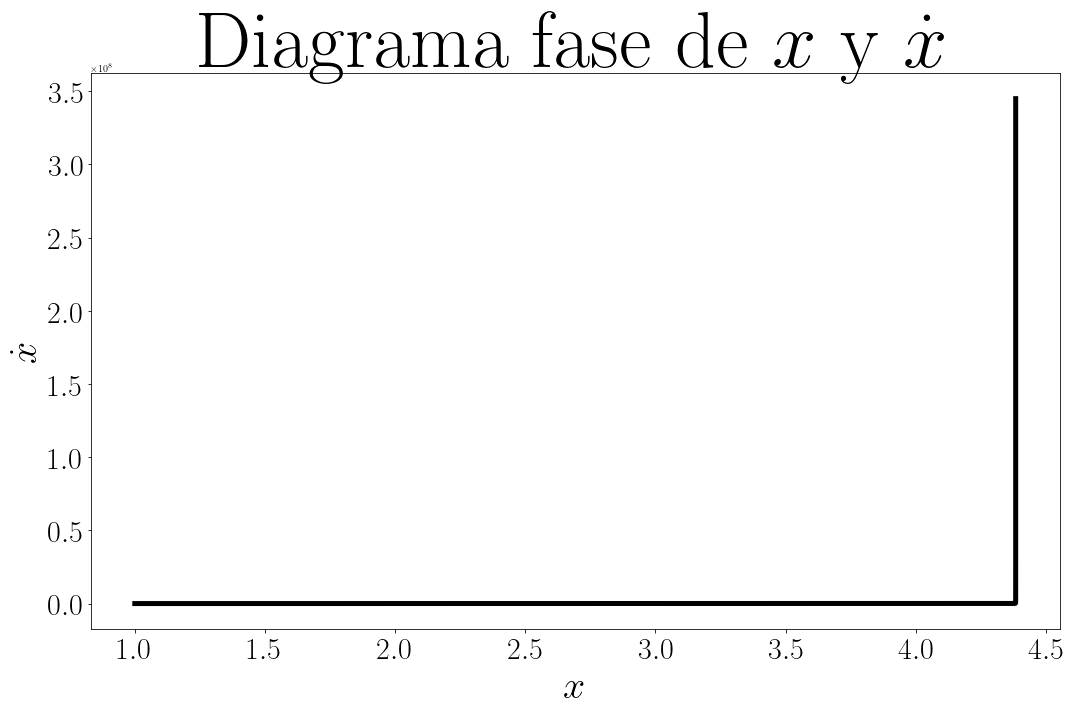
\includegraphics[scale=0.2]{img/sp_phase_x_dx_f0.png}
 % dp_x_theta_f0.png: 1072x712 px, 72dpi, 37.83x25.12 cm, bb=0 0 1072 712
 \caption{Diagrama fase de $x$ y $\dot{x}$ para $F=0$.}
 \label{fig: sp phase x dx force 0}
\end{figure}

\begin{figure}[h]
 \centering
 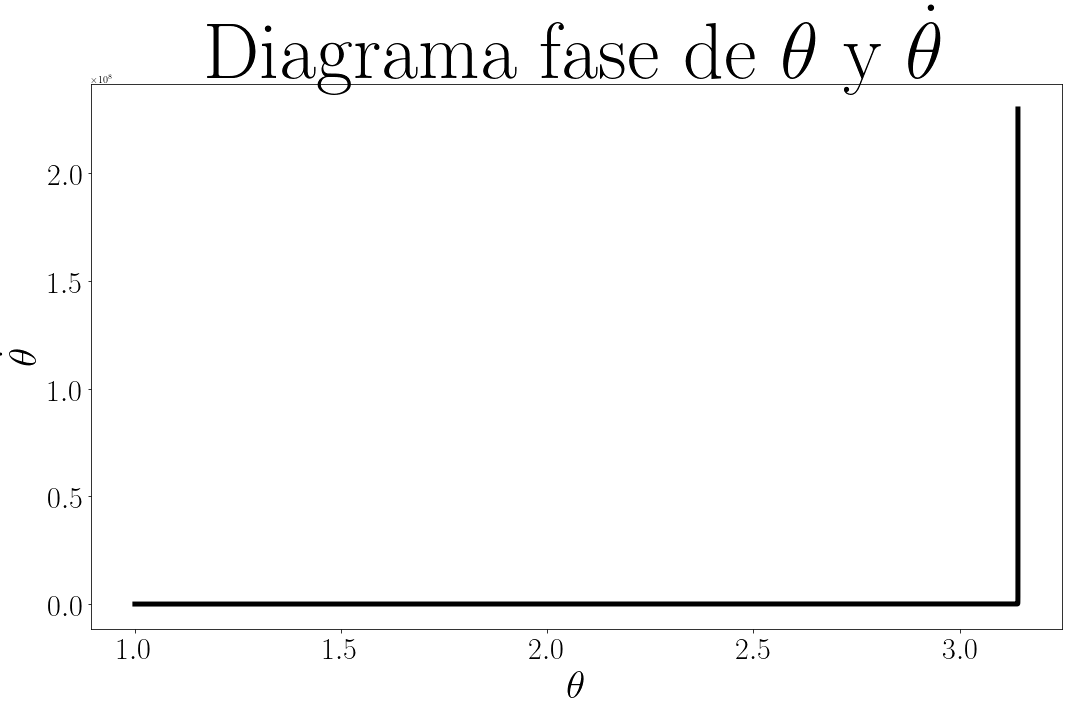
\includegraphics[scale=0.2]{img/sp_phase_theta_dtheta_f0.png}
 % dp_x_theta_f0.png: 1072x712 px, 72dpi, 37.83x25.12 cm, bb=0 0 1072 712
\caption{Diagrama fase de $\theta$ y $\dot{\theta}$ para $F=0$.}
 \label{fig: sp phase theta dtheta force 0}
\end{figure}

\pagebreak

\subsection{Caso 2: $F=1$}

Las figuras \ref{fig: sp x theta force 1} y \ref{fig: sp dx dtheta force 1} muestran el comportamiento del sistema ante la introducción de una fuerza $F=1$. 
Se observa en los diagramas fase de las figuras \ref{fig: sp phase x dx force 1} y \ref{fig: sp phase theta dtheta force 1} que el sistema se comporta de una manera irrazonable, como consecuencia del modelo erróneo que se empleó.

\begin{figure}[h]
 \centering
 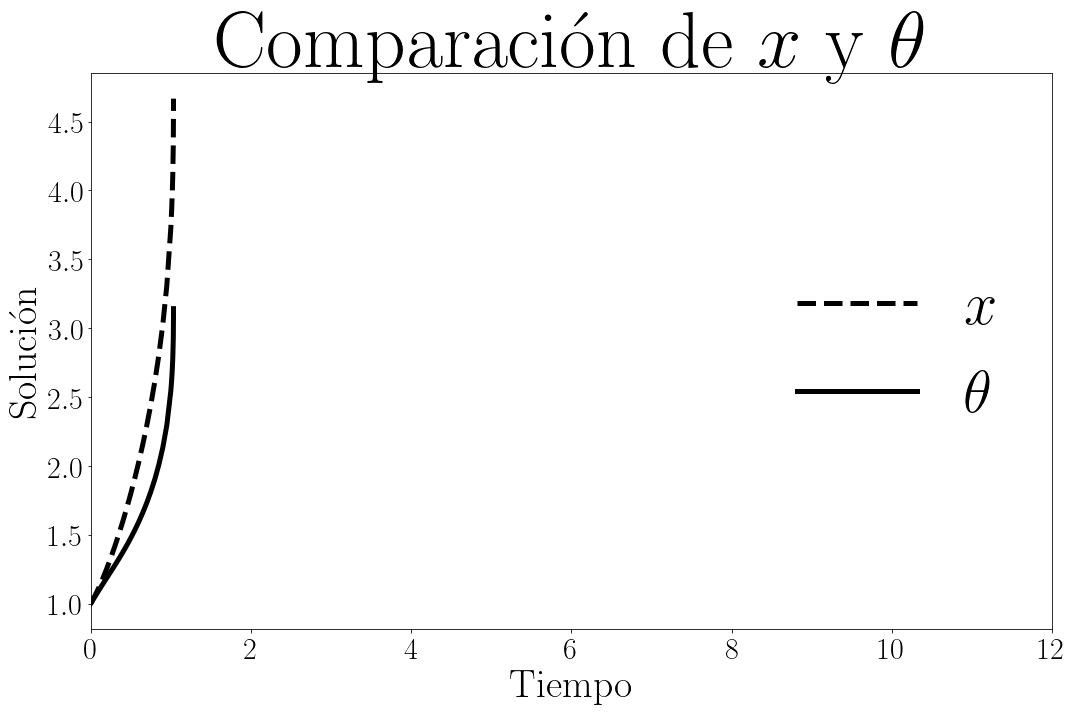
\includegraphics[scale=0.4]{img/sp_x_theta_f1.png}
 % dp_x_theta_f0.png: 1072x712 px, 72dpi, 37.83x25.12 cm, bb=0 0 1072 712
 \caption{Diagramas de $x$ y $\theta$ para $F=1$.}
 \label{fig: sp x theta force 1}
\end{figure}

\begin{figure}[h]
 \centering
 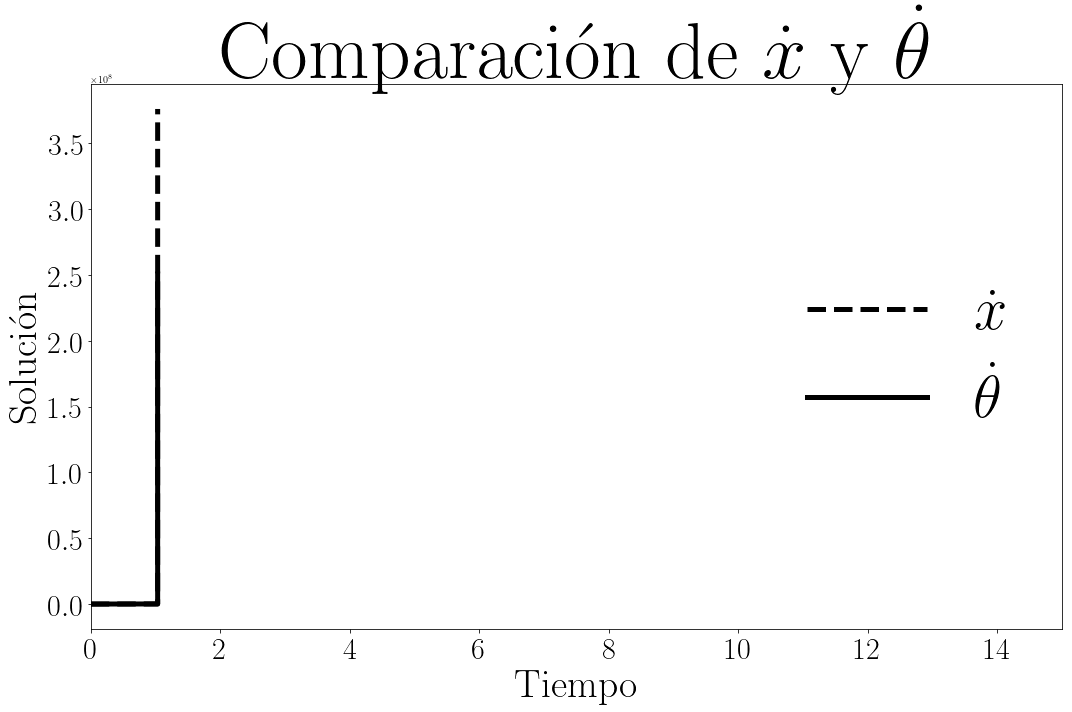
\includegraphics[scale=0.4]{img/sp_dx_dtheta_f1.png}
 % dp_x_theta_f0.png: 1072x712 px, 72dpi, 37.83x25.12 cm, bb=0 0 1072 712
 \caption{Diagramas de $\dot{x}$ y $\dot{\theta}$ para $F=1$.}
 \label{fig: sp dx dtheta force 1}
\end{figure}

\begin{figure}[h]
 \centering
 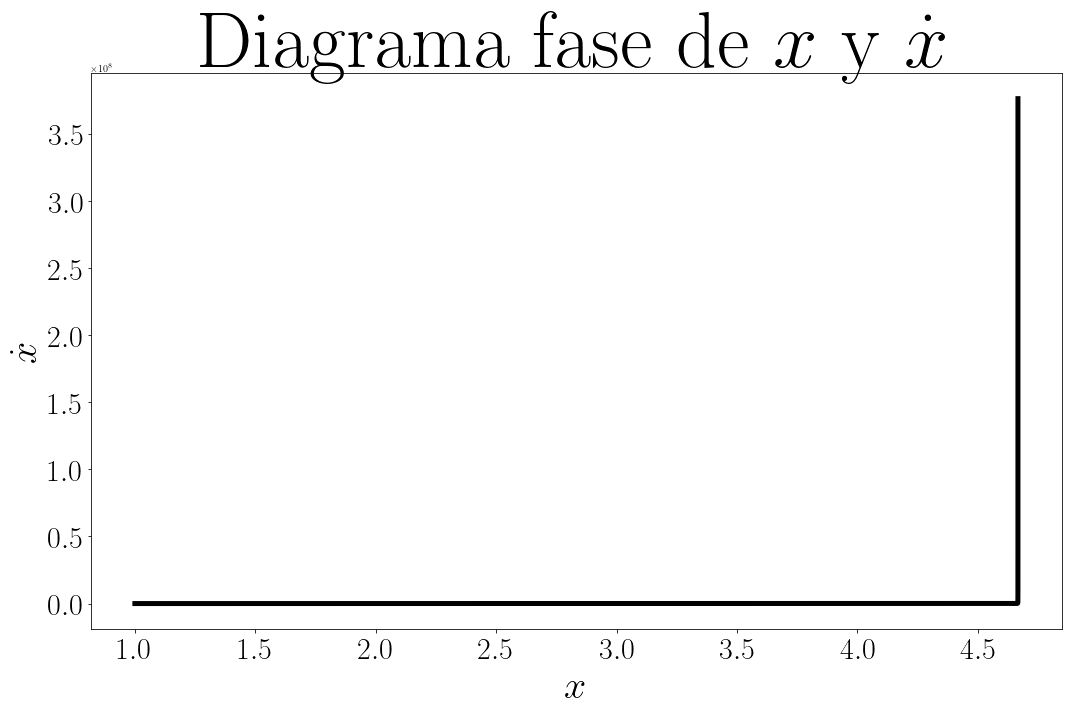
\includegraphics[scale=0.2]{img/sp_phase_x_dx_f1.png}
 % dp_x_theta_f0.png: 1072x712 px, 72dpi, 37.83x25.12 cm, bb=0 0 1072 712
 \caption{Diagrama fase de $x$ y $\dot{x}$ para $F=1$.}
 \label{fig: sp phase x dx force 1}
\end{figure}

\begin{figure}[h]
 \centering
 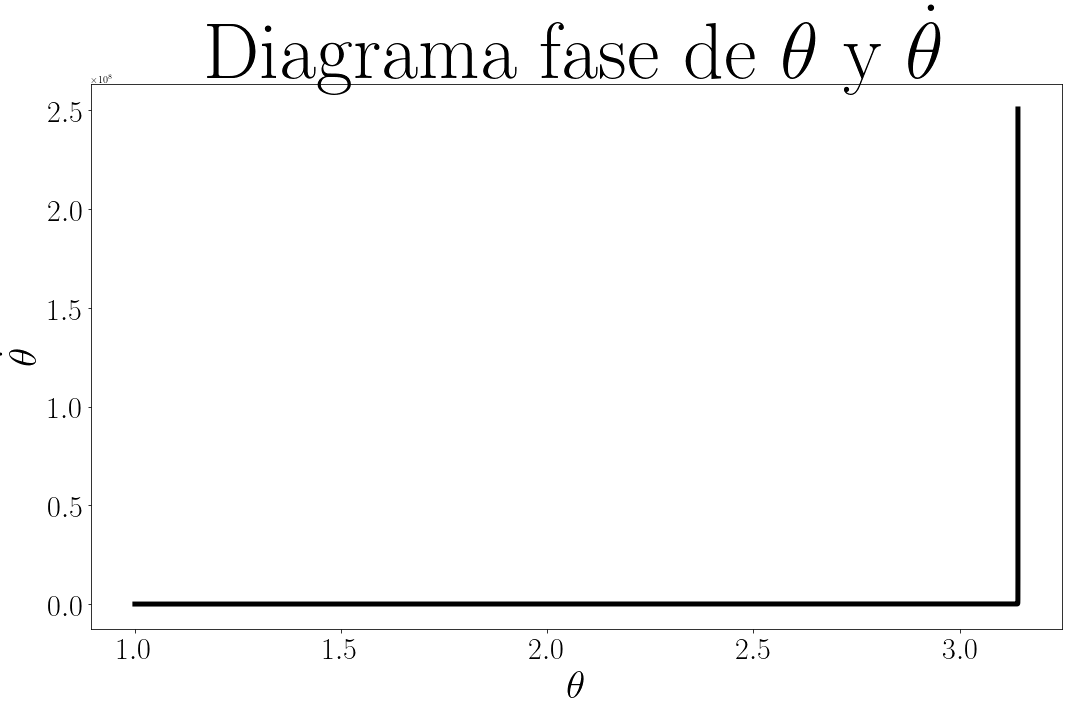
\includegraphics[scale=0.2]{img/sp_phase_theta_dtheta_f1.png}
 % dp_x_theta_f0.png: 1072x712 px, 72dpi, 37.83x25.12 cm, bb=0 0 1072 712
\caption{Diagrama fase de $\theta$ y $\dot{\theta}$ para $F=1$.}
 \label{fig: sp phase theta dtheta force 1}
\end{figure}


\end{document}
